\section{Your First Question Here}

\subsection{Problem}

Describe the problem the interviewee is expected to solve. If applicable
mention constraints like runtime or memory complexity, coding style, edge
cases, etc. If you use information from external sources,
like~\cite{McDowell_Cracking_2015}, consider a citation if it is a book or
article. For blog entries or other links a footnote with a URL will suffice.

\begin{figure}[h]
    \centering
    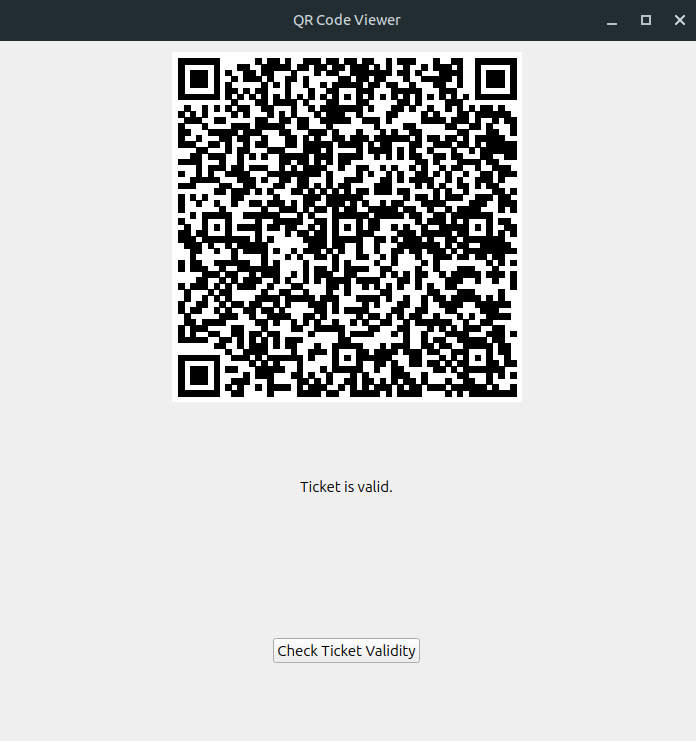
\includegraphics[width=0.44\textwidth]{../figures/QR_Window.png}
    \caption{Example image}
    \label{fig:screenshot}
\end{figure}


\subsection{Baseline Solution}

Give the solution to the previously described problem. Talk about possible
pitfalls and hints you could give the interviewee. Show code snippets where
applicable. You may, of course, also use graphics and plots.

\subsection{(Optional) Post-Interview Experiences}

How was the question received, did interviewees struggle with a particular part
the most.
